\section{Problem resolution}
The first we have done in this project was testing that our program will actually work. As our first coding task we implemented the problem formulation that we described in the section \ref{sec:intro}, the problem reported has only the minimization function and it ensures that each node has only one edge incoming and only one edge outcoming. In this first part of this report, we will consider only the symmetric TSP so the resulting graph will be undirected. Until otherwise specified the following methods are testes with the file \href{http://comopt.ifi.uni-heidelberg.de/software/TSPLIB95/tsp/}{att48.tsp.}

\begin{figure}[h]
	\centering
	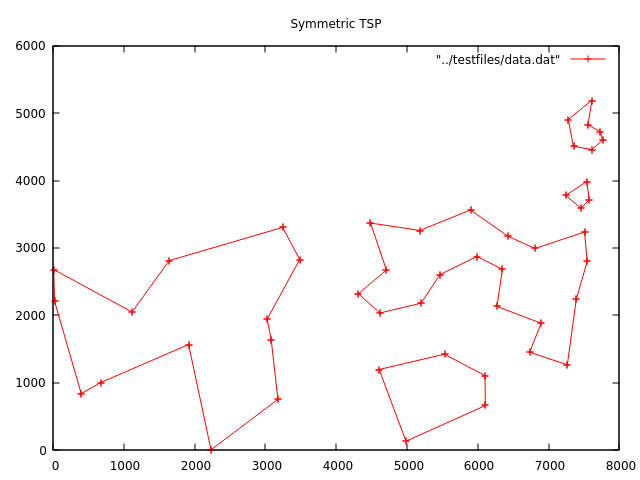
\includegraphics[width=0.6\textwidth]{images/symmetric_with_tours}
	\caption{The image represent att48.tsp solved with the problem formulation showed in section \ref{sec:intro}}
\end{figure}

As we can see the solution that CPLEX found doesn't contain a single tour but a lot of sub-tours. The TSP problem requires that all the nodes must be connected with only one cycle, to do that we implemented different solutions that we will see in this report, the following subsection will explore the basic formulation of the loop method (also known as benders) and some compact models (MTZ and GG).

\subsection{Loop method}
\label{sec:loop}
This method is easier to implement and also easier to understand. This process that we are going to describe is also known as benders decomposition and it is based on the principle of the divide-and-conquer.

%%TODO riscrivere meglio vala'
The basic algorithm is the following: we give CPLEX the same model as before but this time we check if the solution has some sub-tour, if yes then we apply the loop method to each cycle found. Essentially it creates a new constraint and adds it to the problem, the constraint that is going to block the formation of the cycles in the next call of CPLEX. \\
Let's make an example, we have a cycle that is composed by five nodes and consequently by five edges that forms the sub-tour; the constraint we build forces the software to connect those five edges with a maximum of four (number of nodes - $1$) edges, this method must be applied to all the sub-tours found in the solution, then we call again CPLEX to solve the problem. If the problem has again some cycles inside we will apply again the loop method until the nodes are connected with only one cycle.

\begin{figure}[h]
	\centering
	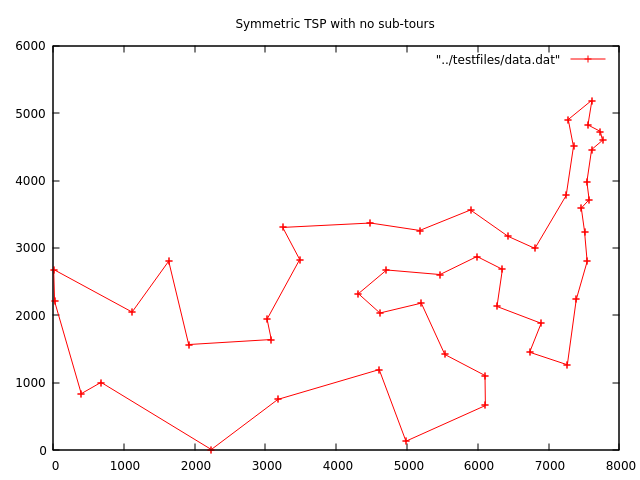
\includegraphics[width=0.6\textwidth]{images/symmetric_with_no_tours}
	\caption{The image represent att48.tsp solved with the loop method described in section \ref{sec:loop}}
\end{figure}

As we can see this time the solution found have no sub-tours and in particular this one was found in circa $0.3$ seconds with a total of 7 iterations where there were added 22 constraints in order to obtain this final solution.

\subsubsection{Particularity of the variable creation in the symmetric TSP}
In the setup section (\ref{cap:2_int}) we have seen how the variable and constraints are implemented inside cplex, we have also seen how we can refer to a variable when using the callable library, by simply using its "position" inside the variable array. It is immediately noticeable that the order in which we create them is really important and allow us to know exactly the position of each variable inside that array.

The way we managed the variables is the following: we think them as they were inside a matrix where the rows are the starting node and the columns are the arriving node. We can see an example in the figure \ref{img:full_matrix}.

\begin{figure}[h]
	\centering
	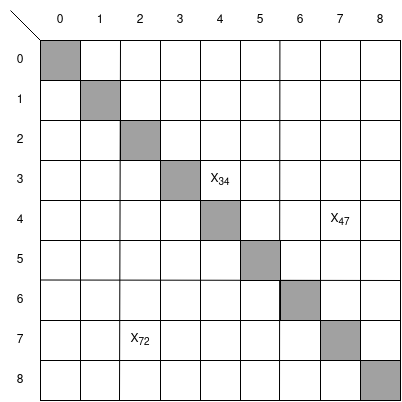
\includegraphics[width=0.55\textwidth]{images/full_matrix}
	\caption{The image represent the matrix method we used to reference the variable inside CPLEX}
	\label{img:full_matrix}
\end{figure}

In this way the is it really simple to find the number of the variable we want to reference, for example if we want to use the index of $x_{34}$ we just need to compute this $3 * (\text{number of nodes}) + 4$ and thats it.

In the particular case of the simmetric TSP the path from $i$ to $j$ and $j$ to $i$ is the same so we don't need all the matrix that we have just showed. So in order to easily obtain the number we image a matrix as the one in the figure \ref{img:full_matrix_simm}, this time all the cells that are in gray are not used since the useful values are saved in the other cells since $x_{ij}$ have the same value than $x_{ji}$.


\begin{figure}[h]
	\centering
	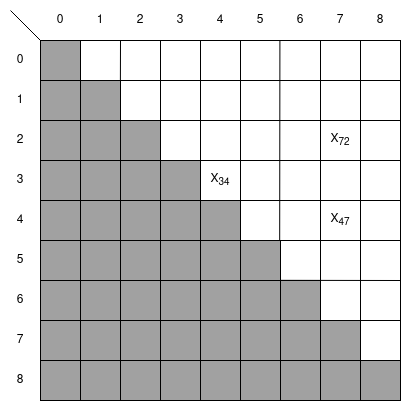
\includegraphics[width=0.55\textwidth]{images/full_matrix_simmetric}
	\caption{The image represent the matrix method we used to reference the variable inside CPLEX in the case of the simmetric TSP. In this case half of the matrix is not used since the values that were in the gray cells are the same of its "corrisponding white cell" since $x_{ij}$ have the same value than $x_{ji}$. In fact the value $x_{72}$ in the figure \ref{img:full_matrix} is transposed into $x_{27}$.}
	\label{img:full_matrix_simm}
\end{figure}
